\section{System Design}

\subsection{Architecture Overview}

EdgeSched adopts a layered architecture design, as illustrated in Figure~\ref{fig:architecture}. The system is divided from top to bottom into presentation layer, domain layer, control plane, execution layer, and data adapter layer. User requests enter the system through WebSocket interfaces, processed by domain layer business logic, then uniformly routed by the control plane to corresponding execution components.

\begin{figure}[!t]
\centering
\IfFileExists{figures/diagrams/system_architecture.pdf}{%
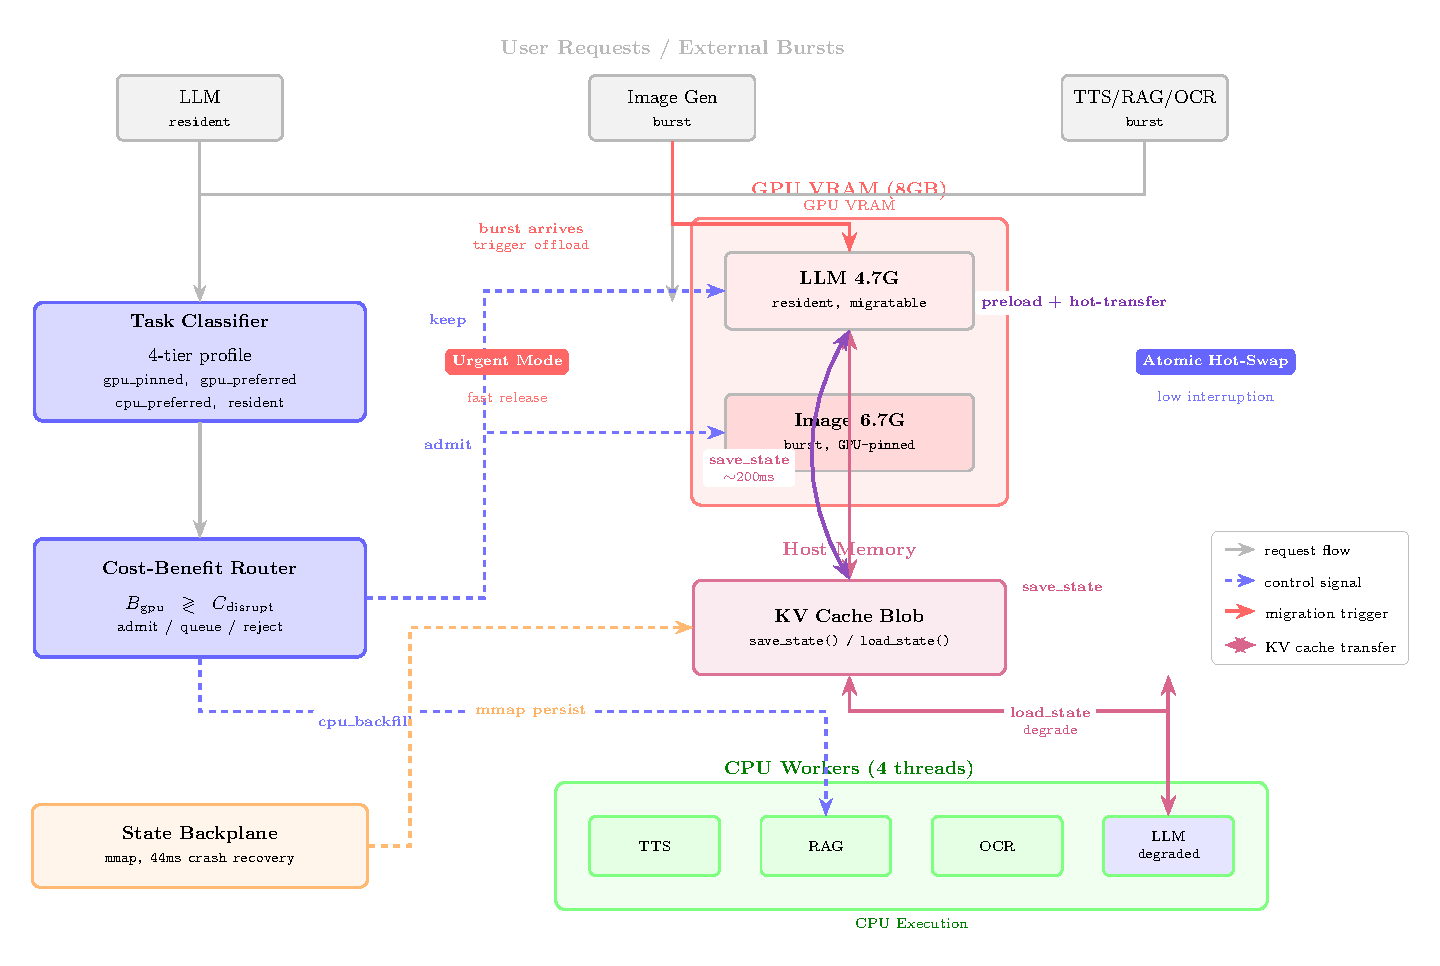
\includegraphics[width=0.95\columnwidth]{figures/diagrams/system_architecture.pdf}%
}{%
\fbox{\parbox{0.92\columnwidth}{\centering System architecture figure unavailable in current workspace build.}}%
}
\caption{EdgeSched system architecture with layered design. The control plane orchestrates task routing while the execution plane manages GPU/CPU resource migration.}
\label{fig:architecture}
\end{figure}

The control plane contains three core components:
\begin{enumerate}
\item \textbf{GlobalTaskScheduler} serves as the L1 routing layer, responsible for task distribution, managing priority queues, cancellation events, and image task backpressure control
\item \textbf{CPPSchedulerEngine} serves as the L2 high-performance execution layer, encapsulating the llama-cpp-python inference engine, implementing GPU/CPU dynamic resource migration
\item \textbf{StateBackplane} implements zero-copy state persistence based on mmap, supporting semantic task-state recovery in about 44ms after crashes
\end{enumerate}

The execution layer contains ResourceManager, responsible for coordinating model lifecycle and GPU/CPU resource allocation, arbitrating resource contention among multiple models. The data adapter layer contains LLM Adapter and Image Adapter, respectively encapsulating large language model (GGUF format) and image generation model (Stable Diffusion) inference logic, shielding differences in underlying inference engines, supporting seamless switching among multiple backends.

\subsection{Dual-Task Scheduling}

EdgeSched instantiates the setting introduced in Section~2 using a concrete high-conflict pair in local AI runtimes: resident, interactive, migratable LLM serving and bursty, GPU-pinned image generation. At the design level, however, the scheduler targets a two-role contention model rather than two hard-coded applications. The first role is a resident service that should remain reachable even under temporary degradation; the second is a burst service that may wait in a queue but should receive exclusive GPU ownership once admitted.

The scheduler therefore treats the two roles differently. In the concrete implementation studied here, LLM requests instantiate the resident role and are directly submitted to CPPSchedulerEngine through \texttt{submit\_llm\_task()}, occupying the GPU by default to maintain low latency. Image-generation requests instantiate the burst role and enter an independent bounded queue through \texttt{try\_enqueue\_image\_generation()}. When a burst task arrives while the resident service occupies GPU VRAM, the scheduler triggers resource migration so that the resident service degrades to CPU execution and the admitted burst task obtains exclusive GPU access. If multiple burst tasks arrive consecutively, subsequent tasks queue, and when the queue is full, the backpressure mechanism rejects new tasks to avoid resource exhaustion and unstable system behavior. Algorithm~\ref{alg:scheduling} presents the core scheduling logic for this two-role model.

\begin{algorithm}[!t]
\caption{Task Scheduling with Backpressure}
\label{alg:scheduling}
\begin{algorithmic}[1]
\STATE \textbf{function} \textsc{SubmitTask}(task)
\IF{task.type == LLM}
    \STATE Submit to CPPSchedulerEngine
    \STATE Allocate GPU by default
\ELSIF{task.type == IMAGE}
    \IF{queue.size() $<$ total\_slots}
        \STATE Enqueue task
        \IF{LLM is on GPU}
            \STATE Trigger \textsc{OffloadToCPU}()
        \ENDIF
    \ELSE
        \STATE \textbf{throw} QueueFullError
    \ENDIF
\ENDIF
\STATE \textbf{end function}
\end{algorithmic}
\end{algorithm}

This design is intended to preserve the availability of the resident service while providing predictable resource allocation for burst tasks.

The design intent is not simply to prioritize one queue over another. Rather, the scheduler treats the two roles as carrying different obligations: the resident service should remain reachable throughout contention, whereas the burst task may wait but should receive exclusive GPU ownership once admitted. This observation drives the control logic in the rest of the section.


\subsection{Design Rationale for Asymmetric Migration}

The key observation behind EdgeSched is that the two directions of migration serve different control objectives. When a bursty GPU-pinned task arrives, the system is under hard VRAM pressure: the immediate objective is to minimize time-to-release so that the GPU can be reclaimed before OOM occurs. In this phase, brief service degradation of the resident task is acceptable, whereas delayed GPU release is not. In contrast, once the burst task completes and VRAM becomes available again, the immediate objective is no longer memory safety but minimizing user-visible interruption while restoring high-performance inference. In this phase, preserving service continuity is more important than minimizing raw reload time.

This asymmetry means that a single symmetric migration routine does not jointly optimize both directions under the same policy in our evaluated setting. If the scheduler is tuned for fast release, it must interrupt promptly and discard the GPU execution context, which helps the GPU$\rightarrow$CPU path but directly harms restoration continuity. If it is tuned for seamless restoration, it must preload in the background and delay cut-over, which helps the CPU$\rightarrow$GPU path but delays reclaiming VRAM when contention arrives. These requirements are therefore in clear tension: ``release fast'' and ``restore without interruption'' are difficult to optimize simultaneously with one shared symmetric policy under hard single-GPU VRAM pressure. The GPU$\rightarrow$CPU path should therefore prioritize fast VRAM release and context preservation, while the CPU$\rightarrow$GPU path should prioritize low-interruption recovery and delayed cut-over. EdgeSched therefore adopts two different policies: \textbf{Urgent Mode} for downlink migration and \textbf{Atomic Hot-Swap} for uplink restoration.

Put differently, the novelty claim of EdgeSched is not that priority queues, model offloading, or state recovery are individually new. The claim is that, on a single memory-constrained device, the two migration directions are governed by \emph{different control objectives}, which creates a strong design trade-off. Under the constraints studied here, a symmetric reload procedure does not jointly achieve the fastest safe downlink and the least disruptive uplink; improving one objective tends to worsen the other. In this sense, asymmetry emerges as a well-justified design choice under the workload constraints rather than as an optional engineering refinement.

\subsection{Dynamic Resource Migration}

Figure~\ref{fig:migration_flow} illustrates the complete resource migration workflow.

\begin{figure}[!t]
\centering
\IfFileExists{figures/diagrams/migration_flow.pdf}{%
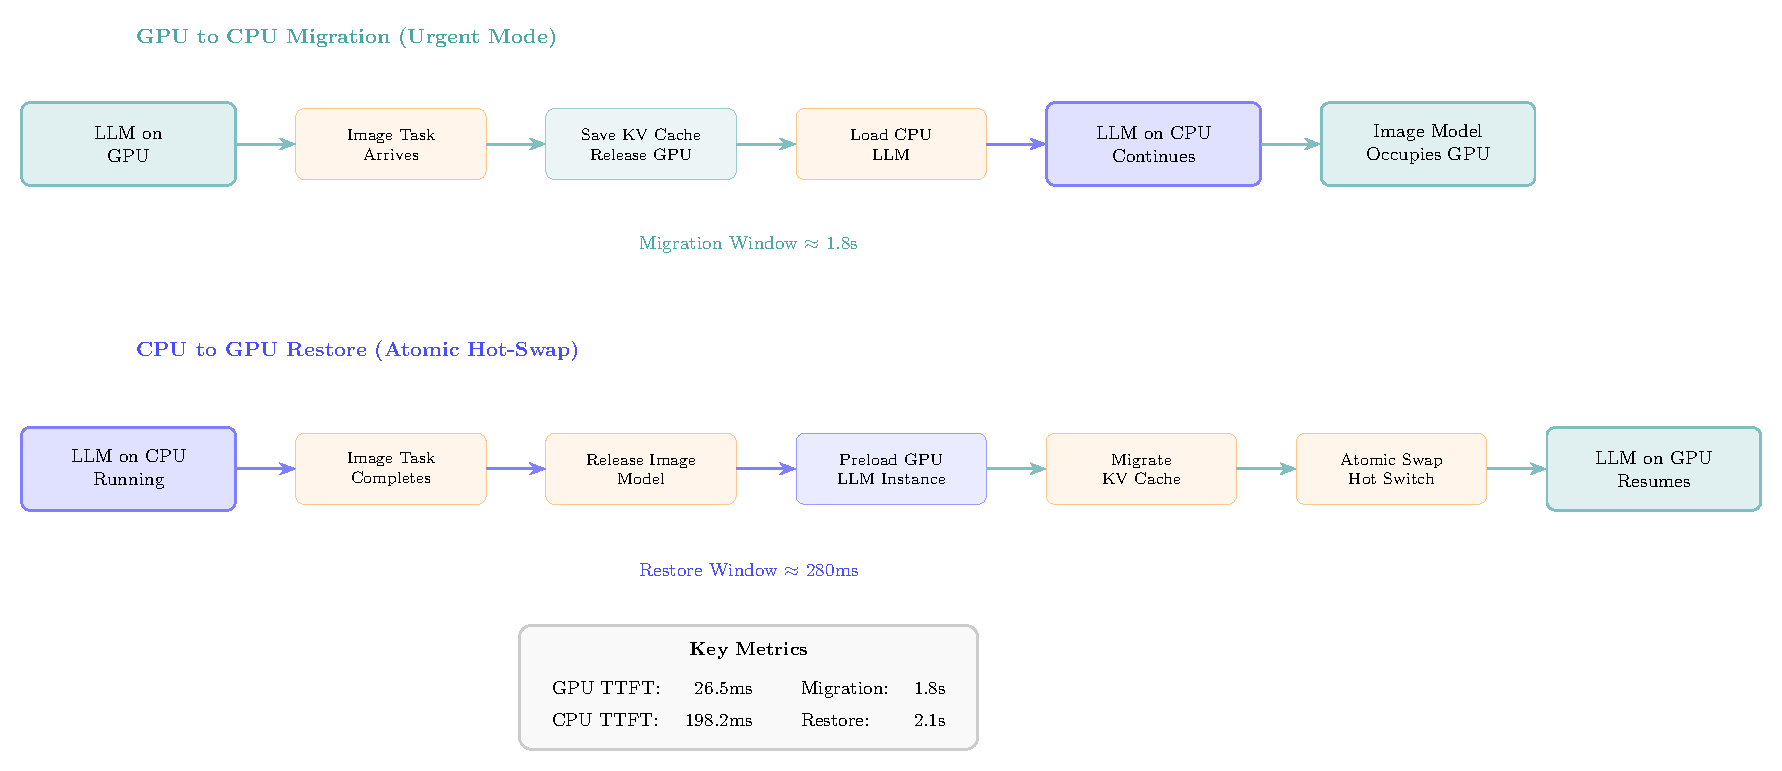
\includegraphics[width=0.95\columnwidth]{figures/diagrams/migration_flow.pdf}%
}{%
\fbox{\parbox{0.92\columnwidth}{\centering Migration workflow figure unavailable in current workspace build.}}%
}
\caption{Resource migration workflow showing asymmetric strategies: Urgent Mode (GPU$\rightarrow$CPU) for rapid preemption and Atomic Hot-Swap (CPU$\rightarrow$GPU) for low-interruption recovery.}
\label{fig:migration_flow}
\end{figure}

\subsubsection{Asymmetric Migration Strategy}

\textbf{Downlink (GPU $\rightarrow$ CPU): Urgent Mode}. When image tasks arrive, the system triggers urgent migration to release VRAM quickly. This policy is optimized for memory safety: it first copies the KV cache from VRAM to host memory through \texttt{save\_state()} (about 200--300 ms in our measurements), preserving conversation context; it then releases GPU allocations so that the image model can be loaded with lower OOM risk. After release, the system starts two operations in parallel: background loading of a CPU LLM instance (helped by the OS page cache) and loading the image generation model to GPU. In other words, Urgent Mode accepts brief performance degradation in exchange for bounded time-to-release.

\textbf{Uplink (CPU $\rightarrow$ GPU): Atomic Hot-Swap}. When image tasks complete and VRAM becomes available again, the system executes atomic hot-swap to restore high-performance LLM inference. This policy is optimized for service continuity rather than immediate cut-over. It adopts a double-buffering strategy:
\begin{enumerate}
\item \textbf{Preload}: First load a fresh LLM instance on GPU while the CPU instance continues serving user requests
\item \textbf{Hot Transfer}: Once the GPU instance is ready, briefly pause the CPU instance, extract the KV cache through \texttt{save\_state()}, and load it into the GPU instance
\item \textbf{Switch \& Unload}: Finally atomically replace the active instance pointer, route new requests to the GPU instance, and asynchronously unload the CPU instance
\end{enumerate}

In our implementation, this mode limits the user-visible interruption during restoration to the final state-transfer and cut-over window, rather than the full GPU reload time. Conceptually, this design is closer to established availability-oriented techniques such as preloading and delayed cut-over than to a claim of inventing a new low-level primitive~\cite{cully2008remus}. What EdgeSched contributes is the decision to apply such a continuity-oriented policy only on the uplink path, while using a more aggressive memory-safety policy on the downlink path.

\subsubsection{Implementation Mechanisms}

Asymmetric migration implementation relies on three core mechanisms:
\begin{enumerate}
\item \textbf{Concurrency Control}: \texttt{asyncio.Lock()} keeps instance replacement atomic and reduces race-condition risk
\item \textbf{State Serialization}: llama-cpp-python's \texttt{save\_state()} / \texttt{load\_state()} interfaces are used to migrate KV-cache state between GPU-backed and CPU-backed instances
\item \textbf{Async Cleanup}: Background release of old instances through \texttt{asyncio.create\_task()} avoids blocking the main service path
\end{enumerate}

\subsection{Backpressure Control}

Image generation tasks are computationally intensive with large VRAM occupation; the system adopts bounded queues to prevent resource exhaustion. Image queue capacity is jointly determined by \texttt{queue\_capacity} (default 8) and \texttt{max\_concurrent} (default 1), with total slots being their sum (default 9). \texttt{max\_concurrent} represents concurrent execution count, \texttt{queue\_capacity} represents queued waiting count.

Queue management is implemented through \texttt{try\_enqueue\_image\_generation()}: the system uses \texttt{asyncio.Queue(maxsize=total\_slots)} to create a bounded queue; if the queue is not full, tasks enqueue for execution; if full, it raises \texttt{RuntimeError("Image queue is full")} to reject requests. This design aims to keep system behavior predictable under high load, rather than allowing unbounded task accumulation that can worsen memory pressure and response latency.

Additionally, the system tracks image task states (pending/running/completed), supporting task cancellation and result queries, and making task lifecycle state visible to users.

\subsection{Cancellation Semantics}

The system supports users actively canceling executing or queued tasks, adopting cooperative interruption strategies to avoid resource leaks.

\textbf{LLM Streaming Cancellation}. LLM generation adopts streaming output, implementing cooperative cancellation through \texttt{asyncio.Event}. After users call \texttt{cancel\_llm\_request(request\_id)}, the system sets a cancellation flag; the generation loop checks the flag after each token and stops subsequent generation if set. This mode avoids forced termination and reduces the chance of resource leaks.

\textbf{Image Task Cancellation}. Queued image tasks are directly discarded; executing tasks set cancellation flags but cannot be forcibly interrupted (must wait for completion). The system provides cancellation capability through the \texttt{cancel\_image\_job(job\_id)} interface; results of canceled tasks are discarded and not pushed to users.

\textbf{Limitations}. The system does not support hard interruption (forcibly killing GPU tasks), determined by CUDA VRAM management mechanisms. Running image tasks must wait for completion; cancellation only affects whether results are pushed. This design acknowledges the boundary of non-hard-interruptibility, balancing resource safety and response speed.

\subsection{Crash Recovery}

Local deployment environments are unstable; systems may crash due to power outages or exceptions. StateBackplane implements zero-copy state persistence based on mmap, designed to recover task states to a semantically usable state in about 44ms after system restart.

\textbf{Data Layout}. The persistence file size is 1MB, divided into three regions: Header (8B) stores Magic Number and version number for data integrity verification; Task Slots (32 slots, 48B each) store task ID, state, priority, and timestamp; remaining space reserved for expansion.

\textbf{Persistence Mechanism}. When task states change, real-time writing to mmap file through \texttt{register\_task()} and \texttt{update\_task\_status()}. Since mmap directly maps files to memory address space, read/write operations are equivalent to memory access, requiring no traditional I/O data copying, with latency only at microsecond level.

\textbf{Recovery Process}. Upon system restart, StateBackplane initialization reads the persistence file: verifies the magic number and version to ensure correct data format; traverses 32 task slots, extracting active tasks with non-zero states; re-adds Pending-state tasks to the scheduling queue; and marks Running-state tasks as Failed to avoid hanging tasks. This design preserves recoverable task metadata after crashes and provides minimally viable task-closure semantics. Algorithm~\ref{alg:recovery} details the recovery logic.

\begin{algorithm}[!t]
\caption{Crash Recovery Process}
\label{alg:recovery}
\begin{algorithmic}[1]
\STATE \textbf{function} \textsc{RecoverFromCrash}()
\STATE Open mmap file
\IF{magic\_number $\neq$ EXPECTED}
    \STATE \textbf{throw} CorruptedDataError
\ENDIF
\STATE recovered\_tasks $\leftarrow$ []
\FOR{slot in task\_slots[0:32]}
    \IF{slot.state $\neq$ EMPTY}
        \IF{slot.state == PENDING}
            \STATE Re-enqueue to scheduler
        \ELSIF{slot.state == RUNNING}
            \STATE Mark as FAILED
        \ENDIF
        \STATE recovered\_tasks.append(slot)
    \ENDIF
\ENDFOR
\STATE \textbf{return} recovered\_tasks
\STATE \textbf{end function}
\end{algorithmic}
\end{algorithm}
